\documentclass[main.tex]{subfiles}
\graphicspath{{pictures/}}
\begin{document}

\section{Software system design}

The main goals for the software system was the following:
\begin{enumerate}
    \item To separate safety critical and non-safety critical code as much as possible.
    \item Building the non safety critical part to be easily extended and changed without needing to even recompile other parts.
    \item Build the safety critical part as robust as possible by regarding it as a hard real time system.
    \item Have a flexible mission construct that can be sent to the robot to be carried out autonomously.
\end{enumerate}


To begin with we had the software system from last years project (?ref?).
After further examination it was clear that to be able to reach the goals the whole software system
needed to be redesigned and rewritten. A design fulfilling the goals is presented in this section.
First the mission construct is explained in section \ref{sec:mission}.
Second what the big parts are and how the fit together is described in the overview (section \ref{sec:sw_design_overview}),
after this the design of each part is described in detail.

\subsection{The mission construct}
\label{sec:mission}

A mission is constructed as a series of simple tasks that the robot is to carry out to accomplish some work.
For example if the robot have a snowblower accessory attached and we want it to carry out the work of clearing a area of snow a mission like this could be constructed:
\begin{enumerate}
    \item SET ACCESSORY TILT: to 100\%.
    \item GOTO: starting point.
    \item SET ACCESSORY TILT: to 0\%.
    \item ACCESSORY COMMAND: hold shute at $30^o$.
    \item ACCESSORY COMMAND: start blower.
    \item FOLLOW PATH: plow area path.
    \item ACCESSORY COMMAND: stop hold shute.
    \item ACCESSORY COMMAND: stop blower.
\end{enumerate}
In this example mission, first the accessory is tilted up to lift it upp as much as possible.
Then it goes to the starting point. After this it tilts down the accessory, tells the accessory to hold the shute at a angle so the snow is moved to a optimal spot and start the blower.
After the accessory is set up it follows a path that covers the area. When it's done clearing the snow it turns of the parts of the accessory it turned on.
This shows how a mission can be constructed using a list of tasks.

The type of tasks that can be used is given an overview in table \ref{tab:task_types_over} and detailed in the mission executor system in section \ref{sec:mission_executor}.
\begin{table}[H]
    \centering
    \begin{tabular}{| m{3cm} | m{5cm} |}
        \hline
        Task type & Description \\
        \hline \hline
        GOTO & Move the robot to a specific GPS point. \\
        \hline
        FOLLOW PATH & Make the robot follow a path represented as a list of GPS points. \\
        \hline
        WAIT & Wait for a set amount of time. \\
        \hline
        ACCESSORY COMMAND & Send a command to the sccessory. \\
        \hline
        SET ACCESSORY TILT & Tilt the accessory a percentage where 100\% is as furthest from the ground and 0\% is closest to the ground. \\
        \hline
    \end{tabular}
    \caption{Overview of task types.}
    \label{tab:task_types_over}
\end{table}

\subsection{Overview}
\label{sec:sw_design_overview}

\begin{figure}[H]
    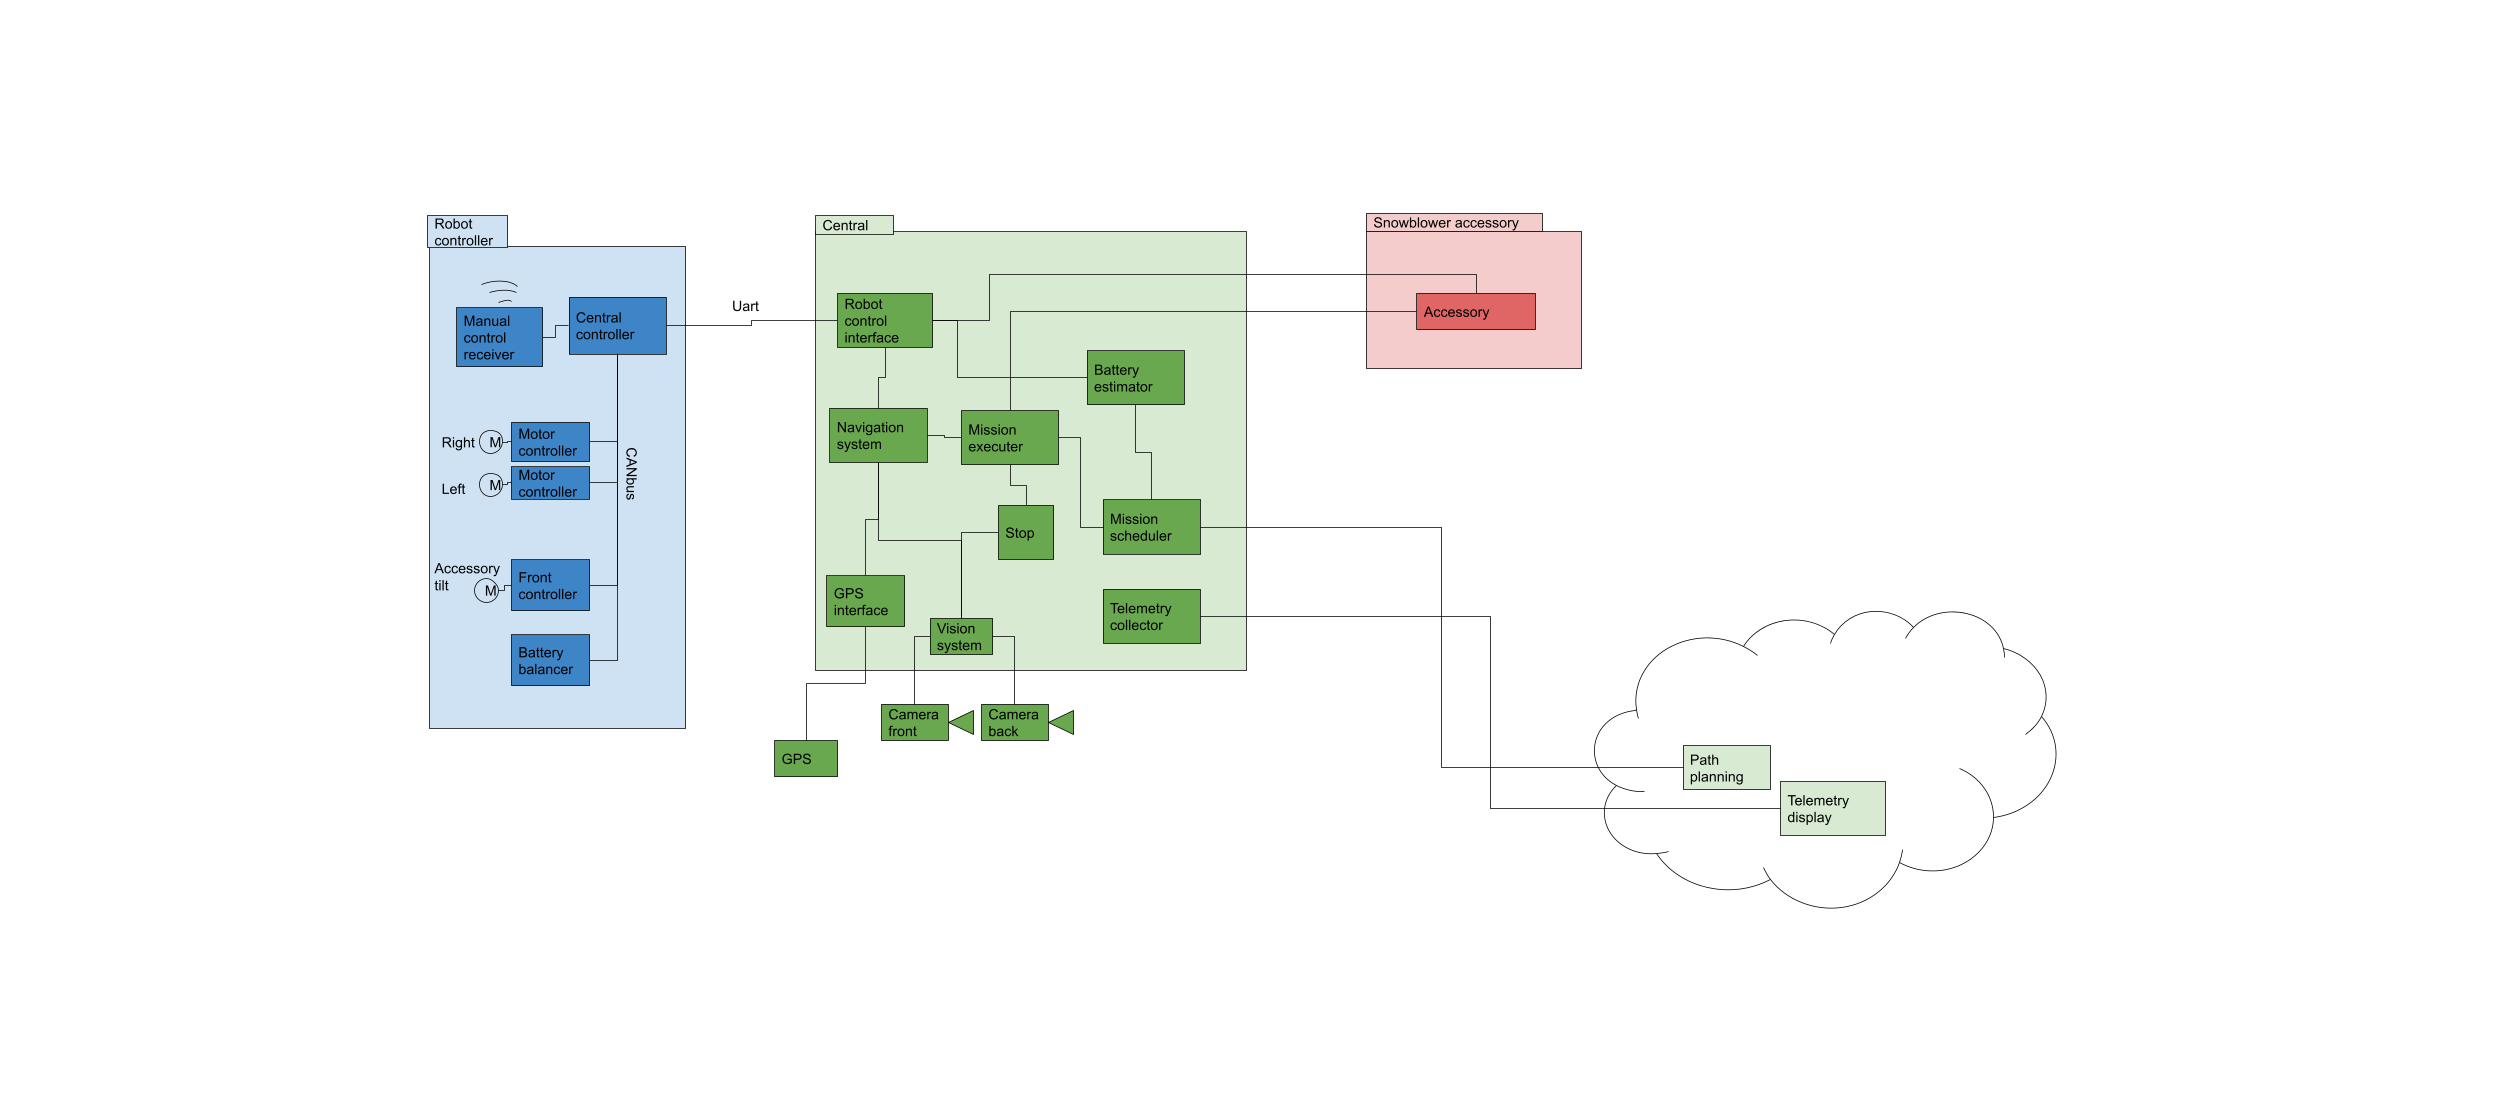
\includegraphics[width=\textwidth]{software_overview.png}
    \caption{Overview of the software architecture.}
    \label{fig:software_overview}
\end{figure}

The design of the software system is made up of different parts and are shown in figure \ref{fig:software_overview}. 
In figure \ref{fig:software_overview} each system is symbolized by a square with a describing name and
lines symbolize communication between systems. Some communication lines are omitted for clarity, what other system each system communicates with is described in the more detailed description of the system design.

The design was divided into 4 main parts, each part has its own color in figure \ref{fig:software_overview}:

The safety critical part is shown in blue and controls the robot directly. 
It's made up of mikrocontrollers running custom firmware written in rust using the RTIC framework (?ref?) except
for the motor controllers that run the Vesc firmware (?ref?).
This systems in this part communicate with each other using one single shared CANbus and communicate with all other systems over a UART link to the robotcontroller interface.

The non safety critical part is shown in the green big rectangle.
This part handles everything needed to do to carry out a mission and sends the proper commands to either the robot controller or the accessory. This part is made up of many interchangeable systems orchestrated in a Arrowhead local cloud (?ref?).

The red part is the accessory, it controls the accessory directly and is a system in the local cloud.
The accessory is designed to be able to be any kind of accessory. In our test case it is a snowblower.

The last part in light green in the little cloud is a separate Arrowhead local cloud running on a server somewhere. It is designed to be the interface between the robot and the world being able to get telemetry from the robot and send missions for it to do.

\subsection{Design of all the parts}

\subsubsection{Mission scheduler}

\subsubsection{Mission executor}
\label{sec:mission_executor}

\end{document}